%start preamble
\documentclass[paper=a4,fontsize=11pt]{scrartcl}%kind of doc, font size, paper size

\usepackage{fontspec}
\defaultfontfeatures{Ligatures=TeX}
%\setsansfont{Liberation Sans}
\usepackage{polyglossia}	
\setdefaultlanguage[spelling=new, babelshorthands=true]{german}
			
\usepackage{amsmath}%get math done
\usepackage{amsthm}%get theorems and proofs done
\usepackage{graphicx}%get pictures & graphics done
\graphicspath{{pictures/}}%folder to stash all kind of pictures etc
\usepackage{amssymb}%symbolics for math
\usepackage{amsfonts}%extra fonts
\usepackage{caption}%captions under everything
\usepackage{listings}
\numberwithin{equation}{section} 
\usepackage{float}%for garphics and how to let them floating around in the doc
\usepackage{xcolor}%nicer colors, here used for links
\usepackage{dsfont}
\usepackage{stmaryrd}
\usepackage{geometry}
\usepackage{hyperref}
\usepackage{fancyhdr}
\usepackage{multicol}
\usepackage{csquotes}
\usepackage{enumitem}
\usepackage{pythonhighlight}

\usepackage[backend=biber,style=alphabetic,
citestyle=alphabetic]{biblatex} %biblatex mit biber laden
\addbibresource{sources.bib}

%settings colors for links
\hypersetup{
    colorlinks,
    linkcolor={blue!50!black},
    citecolor={blue},
    urlcolor={blue!80!black}
}

\definecolor{pblue}{rgb}{0.13,0.13,1}
\definecolor{pgreen}{rgb}{0,0.5,0}
\definecolor{pred}{rgb}{0.9,0,0}
\definecolor{pgrey}{rgb}{0.46,0.45,0.48}


\pagestyle{fancy}
\lhead{NW+VS -- Übung\\WiSe 2021/22}
\rhead{FB 4 -- IKG \\ HTW-Berlin}
\lfoot{Übungsblatt 03}
\cfoot{}
\fancyfoot[R]{\thepage}
\renewcommand{\headrulewidth}{0.4pt}
\renewcommand{\footrulewidth}{0.4pt}

\lstdefinestyle{Bash}{
  language=bash,
  showstringspaces=false,
  basicstyle=\small\sffamily,
  numbers=left,
  numberstyle=\tiny,
  numbersep=5pt,
  frame=trlb,
  columns=fullflexible,
  backgroundcolor=\color{gray!20},
  linewidth=0.9\linewidth,
  %xleftmargin=0.5\linewidth
}


%%here begins the actual document%%
\newcommand{\horrule}[1]{\rule{\linewidth}{#1}} % Create horizontal rule command with 1 argument of height


\begin{document}
\begin{center}
\Large{\textbf{Übungsblatt 3 -- Einfache verteilte System mit Sockets und HTTP}}
\end{center}

\begin{center}\Large{\textbf{Aufgabe A -- HTTP}}\end{center}\vskip0.25in

Nachdem wir in der letzten Übung bereits erste Erfahrungen mit \emph{HTTP} gemacht haben, wollen wir etwas tiefer in Richtung verteilte Systeme vorstoßen. Dazu nutzen wir weiterhin \emph{HTTP}.
\begin{enumerate}
	\item \emph{HTTP} arbeiten mit Nachrichten in einem Request-Response-Schema. D.h. ein Client sendet Anfragen an den Server, der Server antwortet auf die eingehenden Anfragen.
	\begin{enumerate}
		\item Im Folgenden ist eine \emph{HTTP}-Request abgebildet.
		\begin{figure}[h]
	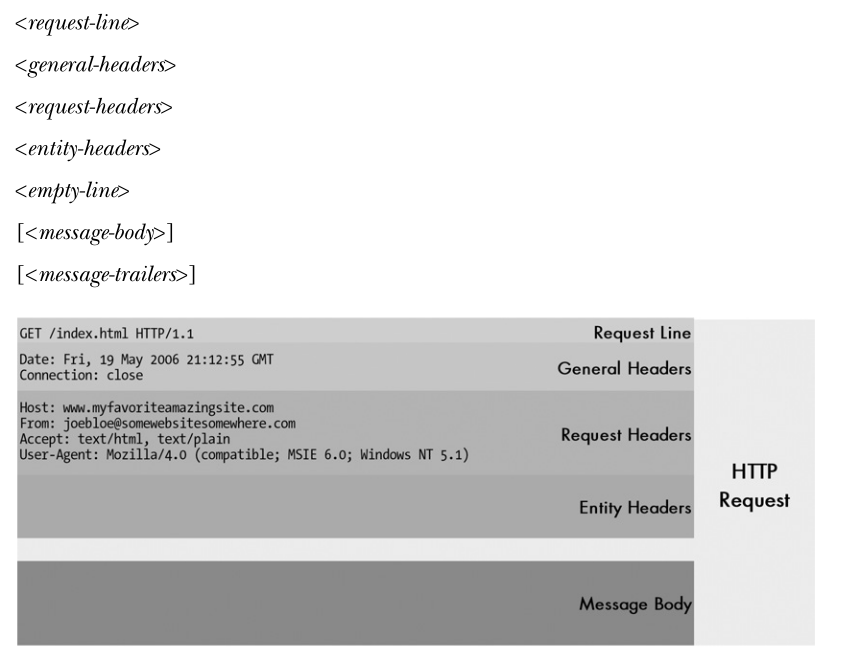
\includegraphics[scale=0.4]{http_req}
	\end{figure}
	Erläutern sie den Aufbau solch einer \emph{HTTP}-Nachricht.
	\item Im Folgenden ist eine \emph{HTTP}-Response abgebildet.
	\begin{figure}[H]
	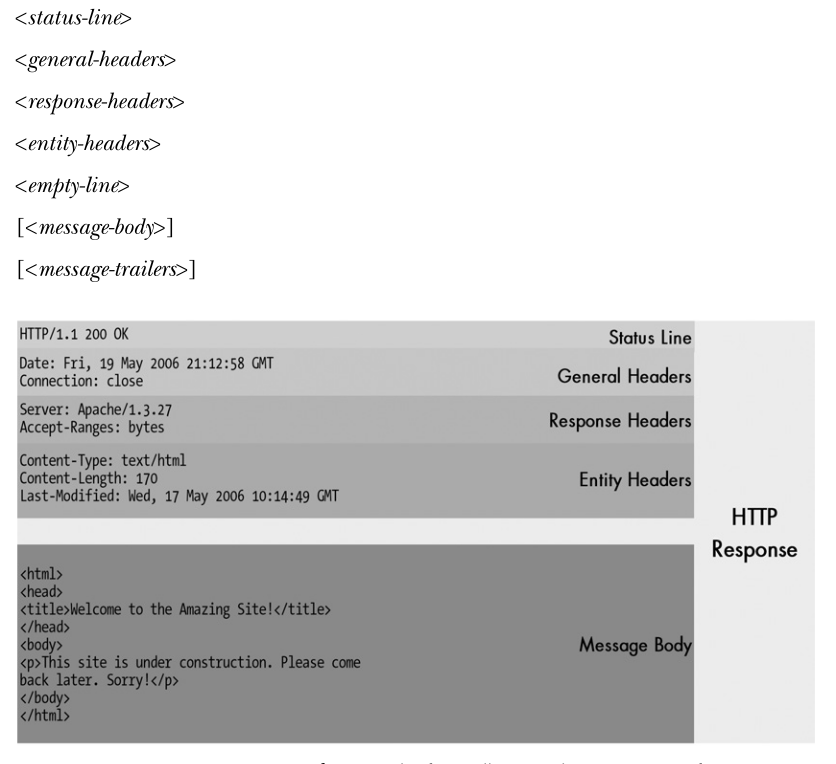
\includegraphics[scale=0.4]{http_resp}
	\end{figure}
	Erläutern sie den Aufbau solch einer \emph{HTTP}-Nachricht.
	\end{enumerate}
	\item \emph{HTTP} ist selbst zustandslos. Jedoch kodiert der Server bei den Antwort auf eine Anfrage die Art der Nachricht.\\
	\emph{HTTP} hat hierbei generell fünf Typen von Codes festgelegt, die erste Ziffer gibt den Typ des Codes an. Recherchieren sie kurz, was folgenden Status-Codes bedeuten:
	\begin{enumerate}
		\item \textit{1yy} 
		\item \textit{2yy}
		\item \textit{3yy}
		\item \textit{4yy}
		\item \textit{5yy}    
	\end{enumerate}
\end{enumerate}

\begin{center}\Large{\textbf{Aufgabe B -- Scapy}}\end{center}\vskip0.25in

In der kommenden Übung arbeiten wir unter anderem mit \emph{Scapy}. Mithilfe von \emph{Scapy} können einfach Pakte gebaut, analysiert und verändert werden. So auch \emph{HTTP}-Pakete.
\begin{enumerate}
	\item Innherhalb \emph{Scapy} können sie sich den Aufbau von verschiedene Paketen anzeigen lassen.
	\item Lesen sie den nachfolgenden Code und kommentieren sie sich, wie ein HTTP-Request und Response umgesetzt werden sollen.
	\begin{python}
>>> load_layer("http")
>>> HTTPRequest().show()
###[ HTTP Request ]### 
  Method    = 'GET'
  Path      = '/'
  Http_Version= 'HTTP/1.1'
  A_IM      = None
  Accept    = None
  Accept_Charset= None
  Accept_Datetime= None
  Accept_Encoding= None
  Accept_Language= None

  [...]
\end{python} 


\begin{python}
>>> HTTPResponse().show()
###[ HTTP Response ]###
  Http_Version= 'HTTP/1.1'
  Status_Code= '200'
  Reason_Phrase= 'OK'
  Accept_Patch43= None
  Accept_Ranges= None
  [...]
\end{python}
\end{enumerate}



\begin{center}\Large{\textbf{Aufgabe C -- Python}}\end{center}\vskip0.25in
Im folgenden ist ein einfacher Chat-Server programmiert.
\begin{enumerate}
	\item Lesen sie den Code zunächst einmal von oben nach unten.
	\item Ein \emph{\#} markiert den Beginn eines Kommentars. Fügen sie an den entsprechen Stellen kommentare ein, die erklären, was der Code macht (an den Stellen, wo \enquote{\# COMPLETE ME} steht).
	
	\begin{python}
import socket # import socket lib -> IP+TCP/UDP
import select # import I/O wait/await etc.
import sys # import OS functionality
from thread import * # threading lib
 
"""The first argument AF_INET is the address domain of the
socket. This is used when we have an Internet Domain with
any two hosts The second argument is the type of socket.
SOCK_STREAM means that data or characters are read in
a continuous flow."""
server = socket.socket(socket.AF_INET, socket.SOCK_STREAM)
server.setsockopt(socket.SOL_SOCKET, socket.SO_REUSEADDR, 1)
 
 
# COMPLETE ME
IP_address = "IP_SERVER"
 
# takes second argument from command prompt as port number
Port = int(PORT)

#COMPLETE ME -> What does 'bind' mean?
server.bind((IP_address, Port))
 
# Max 4 clients can connect to our server
server.listen(4)
# list of client, starting with 0 
list_of_clients = []
 
#def for function start 
def clientthread(conn, addr): # COMMENT ME: what does this function do?
 
    # COMMENT ME
    conn.send("Welcome to this chatroom!")
 
 	# COMMENT ME
    while True:
            try:
                message = conn.recv(2048) # COMMENT ME
                if message:
 
                    # COMMENT ME
                    print ("<" + addr[0] + "> " + message)
 
                    # COMMENT ME
                    message_to_send = "<" + addr[0] + "> " + message # COMMENT ME 
                    broadcast(message_to_send, conn) # COMMENT ME
 
                else: # COMMENT ME
                    """message may have no content if the connection
                    is broken, in this case we remove the connection"""
                    remove(conn)
 
            except:
                continue
 
# COMMENT ME
def broadcast(message, connection):
    for clients in list_of_clients: # COMMENT ME
        if clients!=connection: # COMMENT ME
            try:
                clients.send(message) # COMMENT ME
            except:
                clients.close() # COMMENT ME
 
                # if the link is broken, we remove the client
                remove(clients)
 
"""The following function simply removes the object
from the list that was created at the beginning of
the program"""
def remove(connection):
    if connection in list_of_clients:
        list_of_clients.remove(connection)
 
while True:
 
    """Accepts a connection request and stores two parameters,
    conn which is a socket object for that user, and addr
    which contains the IP address of the client that just
    connected"""
    conn, addr = server.accept()
 
    """Maintains a list of clients for ease of broadcasting
    a message to all available people in the chatroom"""
    list_of_clients.append(conn)
 
    # prints the address of the user that just connected
    print (addr[0] + " connected")
 
    # creates and individual thread for every user
    # that connects
    start_new_thread(clientthread,(conn,addr))    
 
conn.close()
server.close()
\end{python}
	\item Analog zu letzten Aufgabe: Lesen und kommentieren sie den Client-Code.
	\begin{python}
	# Python program to implement client side of chat room.
import socket
import select
import sys

# COMMENT ME
server = socket.socket(socket.AF_INET, socket.SOCK_STREAM) 

# COMMENT ME
IP_address = "IP_CLIENT" # COMMENT ME
Port = int("PORT") # COMMENT ME
server.connect((IP_address, Port)) # COMMENT ME
 
while True:
 
    # maintains a list of possible input streams
    sockets_list = [sys.stdin, server]
 
    """ There are two possible input situations. Either the
    user wants to give manual input to send to other people,
    or the server is sending a message to be printed on the
    screen. Select returns from sockets_list, the stream that
    is reader for input. So for example, if the server wants
    to send a message, then the if condition will hold true
    below.If the user wants to send a message, the else
    condition will evaluate as true"""
    read_sockets,write_socket, error_socket = select.select(sockets_list,[],[])
 
 	# COMMENT ME 
    for socks in read_sockets:
        if socks == server: # COMMENT ME
            message = socks.recv(2048) # COMMENT ME
            print (message)
        else:
            message = sys.stdin.readline() # COMMENT ME
            server.send(message) # COMMENT ME
            sys.stdout.write("<You>") # COMMENT ME
            sys.stdout.write(message) # COMMENT ME
            sys.stdout.flush() # COMMENT ME
server.close() # COMMENT ME
	\end{python}
\end{enumerate}


\printbibliography

\end{document}
